\section{Numerical propagation and normalization}
\label{sec:si-numerics}
All dimensional calculations use millimeters internally, with
$\lambda=0.0006328$ mm and baseline $w=0.08$ mm, hence $kw=794.3344257$.
The envelope amplitude is arbitrary because signals are normalized by
$\mathcal P_{\rm in}$. The original 36 beams use
$m=1,2,3$, $\eta=0.35,0.7$, and
$R_0=24,32,40,56,72,96$. The archived calculation and current implementation
agree in all 432 stored comparisons at their saved precision; numerical
convergence is assessed separately below.

\subsection{Independent implementations}
The source-radius-expanded R-S integral is evaluated with composite Simpson
quadrature in $s=r/w$. A kernel coordinate $y$ is defined by
$a=y/(2R_0)$, $c=[1-(a/kw)^2]^{1/2}$,
$\rho=z a/(kw c)$. Its relation to the physical scaled radius is
$x=z\rho/(2kw^3)$; $y$ is only a computational coordinate.
Bessel functions are evaluated directly for each required integer order.
The source phase is split into a separable part and a small correction
containing $c-1$. Four terms in this correction are retained, with an
absolute exponential-remainder bound evaluated for every grid.
The largest stored bound for the tail correction in the main matrix is
$4.18\times10^{-14}$ in field amplitude; it is not a bound on the
event error, which also depends on signal conditioning.

The independent spectral calculation forms
\begin{equation}
H_q(u)=\int_0^\infty s f(s)J_{|q|}(us)\,\mathrm{d}s,\qquad
U_q(r,\zeta)=\int_0^{u_{\max}}u H_q(u)J_{|q|}(ur)
e^{\ii\zeta\Omega(u)}\,\mathrm{d}u,
\end{equation}
where $r=\rho/w$ and the carrier is removed. The rates are
$\Omega_F=-u^2/2$ and
\begin{equation}
\Omega_{\rm exact}=kw\{[(kw)^2-u^2]^{1/2}-kw\}
=-\frac{u^2kw}{[(kw)^2-u^2]^{1/2}+kw}.
\end{equation}
The forward transform uses a logarithmic Hankel grid on
$10^{-6}\leq s\leq10^4$, with $2^{21}$ points below $R_0=192$ and
$2^{22}$ points at larger radius. The logarithmic increment is computed
from the exact endpoint logarithms, avoiding cancellation in a ratio of
adjacent nearly equal grid points. The inverse transform uses uniform
spectral Simpson integration, including the independently integrated
$u=0$ value for $q=0$, rather than a periodic inverse logarithmic transform.
The retained limit is $u_{\max}=\sqrt{24/\alpha}$, below the grazing
region in these comparisons. Production spectral increments are at most
$0.00125$, $0.000625$, and $0.0003125$ for small, intermediate, and
large radii, respectively.

An independent spatial calculation uses the unexpanded first R-S kernel
\begin{equation}
K(d)=Z\,\frac{e^{\ii kw(d-Z)}}{d^2}
\left(\frac1d-\ii kw\right),\quad
d^2=Z^2+s^2+r^2-2sr\cos\varphi,\quad Z=z/w.
\end{equation}
Angular integration projects the required charge, and radial integration
uses an independent Simpson grid. At $\tau=-0.5,0,1$ and
$x=0,1,3,6$, complex fields are compared on all 17 spectral parameter
sets. The largest relative $L^2$ discrepancy is $4.86\times10^{-8}$.
This agreement concerns the same scalar boundary problem. Reduced R-S,
Fresnel, and exact propagation are model comparisons; exact spectral
versus unexpanded R-S differences are implementation comparisons.

\subsection{Extent, sampling, and event convergence}
The production source grid has $\Delta s\leq0.025$ and
$s_{\max}=R_0+\max(45,c/\alpha)$ with
$c=\lceil16+\alpha R_0\rceil$. A smaller preliminary cutoff was found
insufficient at large $R_0$ and strong apodization. Its omitted tail was
added to the cached channels as a complex amplitude; intensities were
then recomputed including interference. Old data are retained separately.
Full-source versus split-tail calculations at three representative cases
change event positions by less than $8\times10^{-9}$.

Independent convergence axes include source increments $0.04,0.025,0.0125$;
observation counts 301, 601, and 1201 for source quadrature and
201, 401, and 801 for
spectral propagation; and axial steps $0.05$, $0.025$, and $0.0125$ when assessed
on the available nested samples. The spectral forward transform is tested
at $2^{21},2^{22},2^{23}$ points and its inverse increment at
$0.000625,0.0003125,0.00015625$ at $R_0=192$, $\eta=0.2$.
Additional source tails increase $c$ by 2 and 4 at
$(24,0.7),(192,0.2),(256,0.9),(256,1.0)$.
Spectral limits $\sqrt{20/\alpha}$, $\sqrt{24/\alpha}$, and
$\sqrt{28/\alpha}$ are compared by coherent annular corrections,
preserving the stored core field. Each refinement changes one numerical
axis at a time. The two annular spectral-extent changes alter
individual half-heights by at most $6.92\times10^{-9}$ over the
three checked parameter sets.

The final source-tail, spectral-sampling, observation, and axial refinements
give maximum half-height and advance changes of $1.47\times10^{-8}$
and $1.88\times10^{-8}$ in the tested set. A cubic-to-quintic locator
comparison at 27 representative beam cases gives a maximum half-height
change $1.14\times10^{-8}$; stationary-peak changes reach
$9.87\times10^{-7}$, demonstrating that crossing and peak accuracies
are different. A Brent tolerance is not a total numerical error estimate.
All detailed values, including earlier failed convergence levels, are
provided in the source-data tables.

The original two-grid advance change, $4.14\times10^{-7}$, omitted source
extent as an independent axis. Extending that extent changes original
single-order positions by up to $1.45\times10^{-5}$ and advances by
$1.71\times10^{-5}$. Original and revised values are tabulated side by
side. Consequently the former grid estimate is not used as the uncertainty
of the revised calculation. Power convergence alone was also insufficient
to establish event convergence.

\begin{table}[t]
\centering\small
\caption{Different error questions, with representative values in
dimensionless $\tau$. Values from distinct rows are not summed.}
\begin{tabular}{p{.30\linewidth}p{.37\linewidth}p{.22\linewidth}}
\toprule
Quantity & Comparison and scope & Value \\
\midrule
Numerical half-height change & Last isolated representative refinements &
$\leq1.47\times10^{-8}$ \\
Numerical advance change & Same refinement set &
$\leq1.88\times10^{-8}$ \\
Source-extent correction & Original 36 beams; maximum advance change &
$1.71\times10^{-5}$ \\
Single-event model difference & Exact minus reduced; $R_0=192,\eta=0.2,m=4$ &
$-0.05850$ \\
Advance model difference & Same beam and reference $m=1$ &
$-6.92\times10^{-6}$ \\
Fresnel minus reduced advance & Same beam; source-radius/paraxial comparison &
$-4.58\times10^{-9}$ \\
Exact minus Fresnel advance & Same beam; exact longitudinal wavenumber &
$-6.92\times10^{-6}$ \\
Boundary-definition change & $+10\%$ radius; $R_0=24,\eta=0.7,m=4$ &
$+0.009368$ \\
Formal-series residual & $\Delta-(A/R_0+B/R_0^{3/2}+C/R_0^2)$;
$R_0=256,\eta=0.7,m=4$ & $1.70\times10^{-5}$ \\
\bottomrule
\end{tabular}
\end{table}

\section{Boundary continuation and event records}
\label{sec:si-root-events}
Each saved complex field supplies 17 regions: 13 fixed scaled factors
$0.8$, $0.85$, $0.9$, $0.925$, $0.95$, $0.975$, $1$, $1.025$,
$1.05$, $1.075$, $1.1$, $1.15$, $1.2$;
the first actual positive-to-negative $S_3$ zero; a physical radius frozen
at the $m$-dependent proxy value at $z_c$; one common physical radius
given by the $m=1$ proxy at $z_c$; and a raised-cosine soft window.
The soft window is unity below $0.95b_0$, zero above $1.05b_0$, and
transitions continuously between them. Channel powers, their sum and
difference, actual roots, and negative-$S_3$ contributions are all saved.
The identity $Q=T\bar p_3$ is evaluated on the same region and input
normalization; it cannot compare regions with different denominators.

To evaluate boundary sensitivity, we compare $0.9b_0$, $b_0$, $1.1b_0$,
and the first actual positive-to-negative zero. For every boundary and every
order, the first stationary maximum and preceding rising half-height are
reselected from that boundary's own signal. The $m=1$ reference uses the
same construction rule as the target order. Table~\ref{tab:four-boundary-full}
covers all six original radii, both original apodizations, and $m=2,3,4$.
It reports signed advances, absolute changes from $b_0$, signed relative
changes, and actual-root event status. The absolute difference remains the
primary quantity when the reference advance is small.

The postprocessing stores separate statuses for the $Q$ pair, the $T$ pair,
their joint comparison, and continuity of the stored selected-root sequence. Among the
actual-root half-height comparisons, 46 have a defined $Q$ order difference
but no joint Q/T comparison because a required $T$ crossing is unavailable.
These records remain valid for Q-only boundary tables and are not silently
reclassified as missing Q events. Selected-root interruptions are reported separately
from event existence.

The wider $0.8b_0$--$1.2b_0$ family is a stress test, not a replacement
protocol. At $R_0=96$, $\eta=0.7$, the $1.2b_0$ advances are
$-0.006342$, $-0.019772$, and $-0.059266$ for $m=2,3,4$, respectively,
whereas the corresponding $b_0$ events remain positive. This reversal is
retained. It cannot be removed by narrowing the axial window or by calling
the changed aperture a numerical error.

The continuity label is a diagnostic of the stored selected-root sequence.
In the main-text display, adjacent finite roots are connected only when their
separation is at most 0.3 in $x$. A missing root or a larger jump interrupts
that sequence; this does not prove a branch exchange or a discontinuity of
the propagated field. Identifying individual branches through such intervals
would require separate root-continuation data.

\begingroup\scriptsize\setlength{\tabcolsep}{3pt}
\begin{longtable}{rrrccccc}
\caption{Four-boundary half-height advances for the original six radii.\label{tab:four-boundary-full}}\\
\toprule
$R_0$ & $\eta$ & $m$ & $0.9b_0$ & $b_0$ & $1.1b_0$ & \textbf{actual zero} & \textbf{status} \\
\midrule
\endfirsthead
\multicolumn{8}{c}{\tablename\ \thetable\ continued}\\
\toprule
$R_0$ & $\eta$ & $m$ & $0.9b_0$ & $b_0$ & $1.1b_0$ & \textbf{actual zero} & \textbf{status} \\
\midrule
\endhead
24 & 0.35 & 2 & \shortstack{0.07356\\(0.00983, $-11.8\%$)} & \shortstack{0.08338\\(0.00000, $+0.0\%$)} & \shortstack{0.09602\\(0.01264, $+15.2\%$)} & \shortstack{0.08677\\(0.00339, $+4.1\%$)} & BR \\
24 & 0.35 & 3 & \shortstack{0.14966\\(0.02893, $-16.2\%$)} & \shortstack{0.17859\\(0.00000, $+0.0\%$)} & \shortstack{0.21896\\(0.04037, $+22.6\%$)} & \shortstack{0.18733\\(0.00874, $+4.9\%$)} & BR \\
24 & 0.35 & 4 & \shortstack{0.22740\\(0.05732, $-20.1\%$)} & \shortstack{0.28473\\(0.00000, $+0.0\%$)} & \shortstack{0.37116\\(0.08643, $+30.4\%$)} & \shortstack{0.30042\\(0.01569, $+5.5\%$)} & BR \\
24 & 0.70 & 2 & \shortstack{0.09082\\(0.00186, $+2.1\%$)} & \shortstack{0.08896\\(0.00000, $+0.0\%$)} & \shortstack{0.08346\\(0.00551, $-6.2\%$)} & \shortstack{0.08429\\(0.00467, $-5.2\%$)} & D \\
24 & 0.70 & 3 & \shortstack{0.18232\\(0.00423, $-2.3\%$)} & \shortstack{0.18656\\(0.00000, $+0.0\%$)} & \shortstack{0.18377\\(0.00278, $-1.5\%$)} & \shortstack{0.18517\\(0.00139, $-0.7\%$)} & BR \\
24 & 0.70 & 4 & \shortstack{0.27369\\(0.01828, $-6.3\%$)} & \shortstack{0.29197\\(0.00000, $+0.0\%$)} & \shortstack{0.30134\\(0.00937, $+3.2\%$)} & \shortstack{0.30218\\(0.01021, $+3.5\%$)} & BR \\
32 & 0.35 & 2 & \shortstack{0.05671\\(0.00594, $-9.5\%$)} & \shortstack{0.06265\\(0.00000, $+0.0\%$)} & \shortstack{0.07004\\(0.00739, $+11.8\%$)} & \shortstack{0.06464\\(0.00199, $+3.2\%$)} & D \\
32 & 0.35 & 3 & \shortstack{0.11505\\(0.01855, $-13.9\%$)} & \shortstack{0.13361\\(0.00000, $+0.0\%$)} & \shortstack{0.15876\\(0.02515, $+18.8\%$)} & \shortstack{0.13913\\(0.00552, $+4.1\%$)} & BR \\
32 & 0.35 & 4 & \shortstack{0.17414\\(0.03785, $-17.9\%$)} & \shortstack{0.21199\\(0.00000, $+0.0\%$)} & \shortstack{0.26759\\(0.05560, $+26.2\%$)} & \shortstack{0.22216\\(0.01017, $+4.8\%$)} & BR \\
32 & 0.70 & 2 & \shortstack{0.07168\\(0.00446, $+6.6\%$)} & \shortstack{0.06722\\(0.00000, $+0.0\%$)} & \shortstack{0.05867\\(0.00856, $-12.7\%$)} & \shortstack{0.06065\\(0.00657, $-9.8\%$)} & D \\
32 & 0.70 & 3 & \shortstack{0.14382\\(0.00314, $+2.2\%$)} & \shortstack{0.14067\\(0.00000, $+0.0\%$)} & \shortstack{0.12855\\(0.01212, $-8.6\%$)} & \shortstack{0.13230\\(0.00838, $-6.0\%$)} & D \\
32 & 0.70 & 4 & \shortstack{0.21550\\(0.00393, $-1.8\%$)} & \shortstack{0.21943\\(0.00000, $+0.0\%$)} & \shortstack{0.20929\\(0.01015, $-4.6\%$)} & \shortstack{0.21400\\(0.00543, $-2.5\%$)} & BR \\
40 & 0.35 & 2 & \shortstack{0.04648\\(0.00375, $-7.5\%$)} & \shortstack{0.05022\\(0.00000, $+0.0\%$)} & \shortstack{0.05470\\(0.00447, $+8.9\%$)} & \shortstack{0.05144\\(0.00121, $+2.4\%$)} & D \\
40 & 0.35 & 3 & \shortstack{0.09419\\(0.01269, $-11.9\%$)} & \shortstack{0.10687\\(0.00000, $+0.0\%$)} & \shortstack{0.12359\\(0.01672, $+15.6\%$)} & \shortstack{0.11056\\(0.00369, $+3.5\%$)} & BR \\
40 & 0.35 & 4 & \shortstack{0.14231\\(0.02682, $-15.9\%$)} & \shortstack{0.16912\\(0.00000, $+0.0\%$)} & \shortstack{0.20755\\(0.03842, $+22.7\%$)} & \shortstack{0.17621\\(0.00709, $+4.2\%$)} & BR \\
40 & 0.70 & 2 & \shortstack{0.05991\\(0.00577, $+10.7\%$)} & \shortstack{0.05413\\(0.00000, $+0.0\%$)} & \shortstack{0.04413\\(0.01000, $-18.5\%$)} & \shortstack{0.04712\\(0.00701, $-13.0\%$)} & D \\
40 & 0.70 & 3 & \shortstack{0.12027\\(0.00706, $+6.2\%$)} & \shortstack{0.11321\\(0.00000, $+0.0\%$)} & \shortstack{0.09645\\(0.01676, $-14.8\%$)} & \shortstack{0.10240\\(0.01082, $-9.6\%$)} & D \\
40 & 0.70 & 4 & \shortstack{0.18018\\(0.00382, $+2.2\%$)} & \shortstack{0.17636\\(0.00000, $+0.0\%$)} & \shortstack{0.15638\\(0.01998, $-11.3\%$)} & \shortstack{0.16493\\(0.01144, $-6.5\%$)} & D \\
56 & 0.35 & 2 & \shortstack{0.03458\\(0.00142, $-4.0\%$)} & \shortstack{0.03600\\(0.00000, $+0.0\%$)} & \shortstack{0.03744\\(0.00144, $+4.0\%$)} & \shortstack{0.03644\\(0.00044, $+1.2\%$)} & D \\
56 & 0.35 & 3 & \shortstack{0.07004\\(0.00641, $-8.4\%$)} & \shortstack{0.07645\\(0.00000, $+0.0\%$)} & \shortstack{0.08434\\(0.00788, $+10.3\%$)} & \shortstack{0.07821\\(0.00176, $+2.3\%$)} & BR \\
56 & 0.35 & 4 & \shortstack{0.10569\\(0.01497, $-12.4\%$)} & \shortstack{0.12066\\(0.00000, $+0.0\%$)} & \shortstack{0.14105\\(0.02039, $+16.9\%$)} & \shortstack{0.12444\\(0.00378, $+3.1\%$)} & BR \\
56 & 0.70 & 2 & \shortstack{0.04599\\(0.00693, $+17.8\%$)} & \shortstack{0.03906\\(0.00000, $+0.0\%$)} & \shortstack{0.02794\\(0.01111, $-28.5\%$)} & \shortstack{0.03232\\(0.00674, $-17.3\%$)} & D \\
56 & 0.70 & 3 & \shortstack{0.09251\\(0.01081, $+13.2\%$)} & \shortstack{0.08171\\(0.00000, $+0.0\%$)} & \shortstack{0.06094\\(0.02077, $-25.4\%$)} & \shortstack{0.06996\\(0.01175, $-14.4\%$)} & D \\
56 & 0.70 & 4 & \shortstack{0.13873\\(0.01154, $+9.1\%$)} & \shortstack{0.12719\\(0.00000, $+0.0\%$)} & \shortstack{0.09833\\(0.02885, $-22.7\%$)} & \shortstack{0.11220\\(0.01499, $-11.8\%$)} & D \\
72 & 0.35 & 2 & \shortstack{0.02782\\(0.00026, $-0.9\%$)} & \shortstack{0.02808\\(0.00000, $+0.0\%$)} & \shortstack{0.02802\\(0.00006, $-0.2\%$)} & \shortstack{0.02816\\(0.00008, $+0.3\%$)} & D \\
72 & 0.35 & 3 & \shortstack{0.05637\\(0.00321, $-5.4\%$)} & \shortstack{0.05957\\(0.00000, $+0.0\%$)} & \shortstack{0.06304\\(0.00347, $+5.8\%$)} & \shortstack{0.06040\\(0.00083, $+1.4\%$)} & D \\
72 & 0.35 & 4 & \shortstack{0.08504\\(0.00886, $-9.4\%$)} & \shortstack{0.09390\\(0.00000, $+0.0\%$)} & \shortstack{0.10523\\(0.01133, $+12.1\%$)} & \shortstack{0.09603\\(0.00213, $+2.3\%$)} & BR \\
72 & 0.70 & 2 & \shortstack{0.03792\\(0.00732, $+23.9\%$)} & \shortstack{0.03060\\(0.00000, $+0.0\%$)} & \shortstack{0.01925\\(0.01135, $-37.1\%$)} & \shortstack{0.02445\\(0.00615, $-20.1\%$)} & D \\
72 & 0.70 & 3 & \shortstack{0.07643\\(0.01237, $+19.3\%$)} & \shortstack{0.06406\\(0.00000, $+0.0\%$)} & \shortstack{0.04194\\(0.02212, $-34.5\%$)} & \shortstack{0.05281\\(0.01125, $-17.6\%$)} & D \\
72 & 0.70 & 4 & \shortstack{0.11477\\(0.01504, $+15.1\%$)} & \shortstack{0.09973\\(0.00000, $+0.0\%$)} & \shortstack{0.06749\\(0.03224, $-32.3\%$)} & \shortstack{0.08451\\(0.01522, $-15.3\%$)} & D \\
96 & 0.35 & 2 & \shortstack{0.02177\\(0.00065, $+3.1\%$)} & \shortstack{0.02112\\(0.00000, $+0.0\%$)} & \shortstack{0.01992\\(0.00120, $-5.7\%$)} & \shortstack{0.02097\\(0.00015, $-0.7\%$)} & D \\
96 & 0.35 & 3 & \shortstack{0.04414\\(0.00065, $-1.4\%$)} & \shortstack{0.04479\\(0.00000, $+0.0\%$)} & \shortstack{0.04481\\(0.00002, $+0.0\%$)} & \shortstack{0.04494\\(0.00015, $+0.3\%$)} & D \\
96 & 0.35 & 4 & \shortstack{0.06662\\(0.00391, $-5.5\%$)} & \shortstack{0.07053\\(0.00000, $+0.0\%$)} & \shortstack{0.07471\\(0.00418, $+5.9\%$)} & \shortstack{0.07140\\(0.00086, $+1.2\%$)} & BR \\
96 & 0.70 & 2 & \shortstack{0.03055\\(0.00742, $+32.1\%$)} & \shortstack{0.02313\\(0.00000, $+0.0\%$)} & \shortstack{0.01193\\(0.01120, $-48.4\%$)} & \shortstack{0.01780\\(0.00532, $-23.0\%$)} & D \\
96 & 0.70 & 3 & \shortstack{0.06173\\(0.01325, $+27.3\%$)} & \shortstack{0.04847\\(0.00000, $+0.0\%$)} & \shortstack{0.02598\\(0.02249, $-46.4\%$)} & \shortstack{0.03839\\(0.01009, $-20.8\%$)} & D \\
96 & 0.70 & 4 & \shortstack{0.09287\\(0.01736, $+23.0\%$)} & \shortstack{0.07551\\(0.00000, $+0.0\%$)} & \shortstack{0.04168\\(0.03383, $-44.8\%$)} & \shortstack{0.06131\\(0.01420, $-18.8\%$)} & D \\
\bottomrule
\end{longtable}
\noindent\footnotesize Each cell is $\Delta\tau_{50}$ on the first line and $(|\Delta-\Delta_{b_0}|,100(\Delta-\Delta_{b_0})/\Delta_{b_0})$ on the second line. D denotes a defined event and BR a defined event whose stored selected-zero sequence contains an interruption; such cases are not used as one smooth asymptotic branch.
\endgroup


Every positive-to-negative root candidate is retained. The trivial vortex
axis zero is excluded. Initial processing uses a relative $S_3$ floor
$10^{-10}$ and a first-cell exclusion; at four critical cases an
independent axis moment determines $U_q/x^{|q|}$ as $x\to0$.
Spline interpolation of this nonsingular quantity in $x^2$ resolves the
root equation without an intensity floor. It detects no additional root
below the original first radial cell in those cases. This is a numerical
test at stated points, not a proof that every dark root is resolvable.

Root jumps larger than $0.3$ in $x$ break the initial event segments.
Continuation identifiers also match all candidates to their linear
predictions between planes; maximum matching distances $0.15,0.3,0.6$
are audited separately. The 1800 records have unchanged event statuses
and half-height differences below $7\times10^{-16}$ relative to the
initial segmentation. These identifiers label numerical continuations and are not
topological invariants. No spline bridges an absent root or an interrupted
branch. The selected event is the earliest interior positive maximum on
a valid segment; all other extrema and crossing candidates remain in the
archive. If the first segment has no valid peak, later valid segments
are examined explicitly and their interval is reported.

An adaptive extent calculation expands the kernel coordinate to $y=32$
and the axial interval to $[-8,12]$ for
three $R_0=24$ cases with $\eta=0.35,0.7,0.9$, four $R_0=96$
cases with $\eta=0.85,0.9,0.925,0.95$, and $(R_0,\eta)=(256,1.0)$.
Cached inner-field planes are reused;
only new axial planes and the outer annulus are propagated. The wider
search does not supply a universal formation event. In particular,
the actual-root $m=4,6$ events remain unavailable on their valid branches
for the tested $R_0=96$, $\eta=0.9,0.925,0.95$ cases, while
$\eta=0.85$ has defined selected events. Failure of a search and
nonexistence on a particular continuous branch are recorded separately
from propagation failure.

For $\eta=0.7$, $m=4$, the formal leading coefficient multiplying
$(D_1-D_4)/R_0$ is $0.80087525$ for the proxy and $0.45152034$ for the
actual-zero boundary. The finite-radius advances can nevertheless be close:
at $R_0=24$ they are $0.291969$ and $0.302175$. Their subleading terms are
still large, and the actual-root record at that radius contains selected-root interruptions.
On the uninterrupted large-radius branch, the effective coefficients
$R_0\Delta/(D_1-D_4)$ reach $0.75488$ for the proxy and $0.54337$ for
the actual zero at $R_0=256$, moving toward distinct limits. At $R_0=16$,
the actual-root $Q$ pair is defined with $\Delta_Q=0.071292$, but its root
records contain selected-root interruptions; the target-order $T$ rising crossing is absent.
The Q point is therefore shown as a selected-root-interruption point and excluded from the
smooth Q convergence sequence, while the joint Q/T comparison is undefined.
The underlying records are in
\texttt{actual\_proxy\_asymptotic\_comparison.csv}.

Rising fractions $0.1$--$0.9$ are evaluated relative to each region's
own first peak. Same-peak FWHM requires the descending half-height
crossing to precede the next local minimum. Among the 10200 main-matrix
region records, 6530 widths meet this condition, 278 cross half-height
only beyond the next minimum, and 3392 lack a pair of crossings.
The latter two groups remain undefined for same-peak width. The earlier,
less restrictive crossing separation is retained as a separate diagnostic.
Common-window centroids use $[-1,2]$ for every order and require a
continuous defined region there; signed weighting and nearly vanishing
integrals are flagged. First-peak conditioning is reported as
$Q(p)/|Q''(p)|$ and half-height conditioning as $Q(p)/|Q'(h)|$.
They measure sensitivity to specified perturbations, not detector error
without a noise model.

Full-curve registration fits a shift and an amplitude over $[-1,2]$
with a shift search $[-1.9,1.9]$ and reports the remaining relative
$L^2$ shape error. Its interpolation domain stays within the saved
$[-3,5]$ interval. Double ratios instead use $\tau_*=0$ and
$\tau\in[-0.5,0.5]$, requiring all four values above
$10^{-8}$ of the larger peak. A measured regression slope is retained
only as a diagnostic; the analytic slope is never replaced by it.

\section{Higher-order, endpoint, and physical-path checks}
\label{sec:si-residuals}
The analytic $A_m,B_m,C_m$ coefficients follow from polynomial algebra
through $\epsilon^4$ and implicit perturbation of the peak and crossing.
All products of lower-order field terms are retained. The next radial
saddle-amplitude correction can be checked independently using the tilted
Airy moment: with $a=\alpha-\ii u$ and $s_*=R_0-a^2$, it is
$-a/(4s_*^2)=\ii\epsilon^3/16-\ii\epsilon^4t/16+\cdots$.
The $\epsilon^3$ part is a common phase, and the normalized intensity
correction at $\epsilon^4$ is $-\operatorname{Re}(A^*A')/8$.
It changes individual fourth-order events but cancels from the
fourth-order order difference. Algebraic checks across orders give
agreement to $2.8\times10^{-13}$. This check does not fit the generated
$m=4$ difference coefficients to propagation data.

The original derivative-number truncation through $N=4$ is retained as
a baseline truncation comparison. It is not identical to a power series truncated
consistently in $\epsilon$. Its original maximum single-event discrepancy
was $1.639\times10^{-3}$, whereas its representative $m=3$ advance
discrepancy was $1.756\times10^{-3}$. Those are approximation errors,
not quadrature errors. The four original figures and 36 parameter cases
define the baseline comparison set.

The formal coefficients are compared without fitting on all available
main-grid radii. Separate least-squares diagnostics fix $A_m$ and fit
$B_m,C_m$ using $R_0\leq96$; the held-out radii are $128,192,256$.
The fit coefficients are labelled empirical and kept separate from
formal coefficients. Near a degenerate Airy maximum, large higher-order
coefficients and finite-radius peaks do not validate a nondegenerate
asymptotic event. At $\eta=1$, the finite-radius proxy events are
retained but no continuation of the simple leading Airy event is asserted.

The fourth-order series at \(\eta=0.35\) does not uniformly improve the
smallest radii and does not locate the intermediate-radius minimum. The
focused calculation in Sec. 14 now closes this residual for \(m=3\): a
compact Airy identity reproduces the full propagated signal, and its
non-fitted expansion through fourteenth order predicts the minimum at
\(R_0=36.37128\), compared with \(36.37130\) for reduced R-S
propagation. The missing fifth- and sixth-order coefficients contain
both field products and nonlinear event terms. This result supersedes
the earlier unresolved attribution for the fixed-proxy \(m=3\) event; it
does not turn a partition-dependent endpoint or Hankel component into an
independently measurable power. The earlier \(m=4\) and other-parameter
comparisons remain finite-order diagnostics with their stated scope.

To examine omitted spectral contributions, the source-axis neighborhood
is smoothly removed from individual Hankel branches below $R_0-10$
and restored through a transition ending at $R_0-8$. A high-frequency
partition is zero below $u_a=\sqrt{R_0}/d$ and one above $2u_a$,
with raised-cosine transition and $d=6,4,3$. The inward and outward
Hankel transforms are propagated coherently; $(1-\chi)H_q$ defines
the low-frequency endpoint component. The remaining high-frequency
field is retained as an explicit remainder. The Debye transform with
8 and 12 terms is checked against direct Hankel-function integration.
Individual components depend on the chosen partition, so their squared
norms are not additive powers and cannot uniquely allocate a physical
mechanism to the residual.

For $\eta=0.7$, $m=4$, $R_0=24$, removing the endpoint component
changes the advance by between approximately $-0.0239$ and $+0.0132$
across the three partitions. At $R_0=256$, the corresponding changes
are between $-4.79\times10^{-5}$ and $+1.04\times10^{-5}$.
The outward component is smaller in field norm at these cases, but
cannot be ignored merely because it has no inward stationary point.
The full coherent sum is partition independent to the implementation
accuracy. Additional $\eta=0.35$ calculations at $R_0=24,32,40,56$
test the nonmonotonic-residual region without changing its data or
analytic coefficients.

The 61 extended parameter jobs contain 276 beams: 40 high-order controls
including $m=1,8,12,16$; 16 small-ring cases at $R_0=8,12$;
88 generalized-$P$ beams; 60 fixed-$\alpha$ beams; and 72 varying-$kw$
beams. High-order searches use a wider radial observation range and
$-6\leq\tau\leq8$. At fixed $\alpha=0.02,0.04,0.07$,
$\eta$ varies with $R_0$ rather than remaining on the principal
asymptotic path. Twenty fixed-$\alpha$ beams have no selected proxy
peak in their stated search interval. They remain in the tables.
No additional validity range is inferred merely from a successful run.

For $P=2,3$, let $h_P$ be the reference event with $m=P$.
The derived leading difference is
\begin{equation}
h_P-h_m=\frac{K_\gamma[\tau](N_{P,P}-N_{P,m})
+K_\gamma[|A'/A|^2](L_{P,P}-L_{P,m})}{R_0}+\cdots.
\end{equation}
At $\eta=0.7$, $P=2,m=4$, its coefficient is $4.61595486$;
the computed difference at $R_0=192$ is $0.02490738$, compared with
the leading $0.02404143$. For $P=3,m=5$, the coefficient is
$4.30569959$ and the corresponding values are $0.02477906$ and
$0.02242552$. These finite-radius discrepancies are retained.
The $m<P$ controls also have positive advances relative to $m=P$
in the sampled set, so monotonicity with $m$ from the adjacent-order
$P=1$ proof is not a general-$P$ statement.

\section{Maxwell completion and longitudinal diagnostics}
\label{sec:si-maxwell}
Let $a=m-1$, $b=m+1$, $\kappa=\sqrt{(kw)^2-u^2}$ and suppress
the common propagation exponential in the integrals below. Preserving
the specified transverse spectrum gives
\begin{align}
E_z(r,\theta)&=\frac{\ii e^{\ii m\theta}}2
\int u^2\frac{H_b-H_a}{\kappa}J_m(ur)e^{\ii\zeta\Omega}\,\mathrm{d}u,\\
V_a(r)&=\int u\left[\frac{\kappa}{kw}H_a+
\frac{u^2(H_a-H_b)}{2kw\kappa}\right]J_a(ur)e^{\ii\zeta\Omega}\,\mathrm{d}u,
\end{align}
with $V_b$ obtained by interchanging $a,b$.
Writing magnetic fields in impedance-scaled units,
\begin{align}
Z_0H_x&=\tfrac\ii2(V_be^{\ii b\theta}-V_ae^{\ii a\theta}),&
Z_0H_y&=\tfrac12(V_ae^{\ii a\theta}+V_be^{\ii b\theta}),\\
Z_0H_z&=-\frac{e^{\ii m\theta}}{2kw}
\int u^2(H_a+H_b)J_m(ur)e^{\ii\zeta\Omega}\,\mathrm{d}u.
\end{align}
The axial Poynting flux obeys
$2Z_0\langle S_z\rangle=\operatorname{Re}(U_aV_a^*+U_bV_b^*)/2$.
This completion differs from projecting a guessed three-component
input and thereby changing the prescribed transverse channels.

The 27 beam/waist cases combine $(R_0,\eta)=(24,0.7),(192,0.2),
(256,0.9)$, $kw=200,800,1600$, and $m=1,4,6$.
Seven common planes $\tau=-1,-0.5,0,0.5,1,1.5,2$ are sampled.
The electric longitudinal fraction is
$\int_{\rm ROI}|E_z|^2/\int_{\rm ROI}(S_0+|E_z|^2)$.
Maximum local fractions use declared bright-pixel masks
$S_0>10^{-9}S_{0,\max}$ and $10^{-6}S_{0,\max}$.
Full-plane retained transverse power, Stokes imbalance, and flux are
reported separately from ROI quantities. The retained transverse power
agrees with the incident scalar normalization to approximately $10^{-9}$
in the checked cases. Apparent remote FFTLog wrap tails are not interpreted
as physical grazing-angle content.

At $R_0=256$, $\eta=0.9$, $kw=800$, the largest sampled relative
ROI axial-flux correction over the three orders is approximately
$1.91\times10^{-4}$. The sampled maxima of the longitudinal electric
fraction across the three physical cases rise from
$3.37\times10^{-5}$--$3.70\times10^{-4}$ at $kw=800$ to
$5.40\times10^{-4}$--$5.77\times10^{-3}$ at $kw=200$.
Small values in these cases do not establish a universal bound near
dark pixels, high orders, or tighter focusing.

Independent Cartesian spectral integration enforces
$\bm k\cdot\widetilde{\bm E}=0$ and
$Z_0\widetilde{\bm H}=\bm k\times\widetilde{\bm E}/k$ directly.
Angular resolutions 64,128,256 agree with the radial recurrence formulas
at matched quadrature points to relative $E,H$ error below
$1.4\times10^{-12}$ and relative $E_z$ error below $6.3\times10^{-12}$.
Comparison to stored interpolated radial fields instead gives errors
up to $1.48\times10^{-7}$, which include interpolation and differing
spectral increments. Operator verification and grid verification are
therefore reported separately.

\section{Input mismatch and two-dimensional controls}
\label{sec:si-inputs}
The input-tolerance study uses $R_0=24,96$, $\eta=0.35,0.7$,
$m=1,2,4$ on $[-8,8]$. Signed power imbalance weights the two
channels by $\sqrt{1+\delta}$ and $\sqrt{1-\delta}$, with
$\delta=\pm0.005,\pm0.01,\pm0.02,\pm0.05$.
Differential radial scales use $f(s/(1\pm\delta/2))$ with
$\delta=\pm0.01,\pm0.02$. Differential ring radii use
$R_\pm=R_0(1\pm\delta/2)$ with $\delta=\pm0.005,\pm0.01$;
$w$ and $\alpha$ remain fixed. Each distorted radial channel is
normalized back to its specified input power, so power imbalance is
not silently added to a geometric mismatch.

Differential quadratic phase is imposed as
$\exp[\pm\ii\beta(s/R_0)^2/2]$ with $\beta=\pm0.1,\pm0.3$ rad.
This is a spatial phase error at the input, distinct from a uniform
post-propagation channel phase. Common scale changes $0.99,1.01$,
a common quadratic phase, and source apertures at $1.5,2,3$ times
$r_0$ are controls. The finite aperture uses a raised-cosine transition
of width $0.5w$; transmitted input power is recalculated and retained.
All events use the nominal proxy aperture. This protocol does not
claim to track a deformed actual-zero contour for a nonaxisymmetric beam.

\begin{figure}[t]
\centering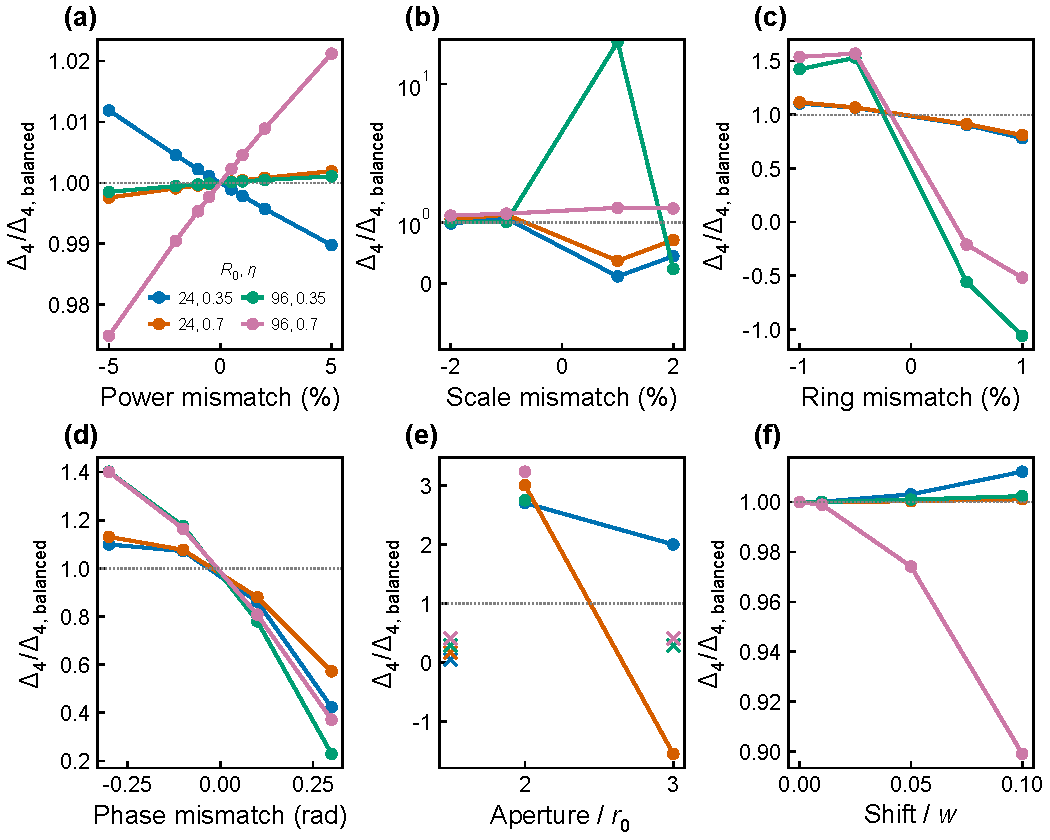
\includegraphics[width=\linewidth]{../figures/input_sensitivity.pdf}
\caption{Input sensitivity of the nominal-proxy $m=4$ advance, divided
by the corresponding balanced-input value. The legend gives $R_0,\eta$.
(a) Signed power imbalance. (b) Differential radial scale; a symmetric
logarithmic vertical axis retains large branch-dependent changes.
(c) Differential ring radius. (d) Differential quadratic phase at $r_0$.
(e) Finite source aperture; crosses denote undefined paired advances
and their vertical positions carry no numerical meaning.
(f) Displacement of the plus channel in a two-dimensional calculation.
These perturbation levels are tests, not accepted hardware tolerances.}
\label{fig:si-input}
\end{figure}

The 324 beam cases yield 315 defined selected peaks and nine cases
without a peak in the search interval, all involving the smallest source
aperture. Six further selected peaks lack a preceding half-height crossing.
In total, 309 individual half-heights and 304 paired advances are defined;
five additional differences lack the reference crossing. Missing
quantities retain separate peak, crossing, and paired-event statuses. The large change at $R_0=96$, $\eta=0.35$, positive radial
scale mismatch is retained together with its complete extrema list;
it cannot be interpreted as a small linear tolerance coefficient.

Finite source apertures can produce very weak early lobes, which remain
eligible under the declared first-peak rule. For $R_0=24$, $\eta=0.7$ and
a source aperture $3r_0$, the selected $m=1,4$ peaks occur near
$\tau=-6.11457,-5.68705$, well before the largest caustic peak. A three-level
source, radial, and axial refinement changes their last half-heights by
less than $1.3\times10^{-8}$ and their difference by less than
$2.3\times10^{-8}$. The $m=2$ preceding half-height remains missing in
that search window. Thus the large aperture-induced changes are not
interpreted as small shifts of a uniquely tracked caustic peak.

Translations are implemented by the translation invariance of the exact
scalar propagator applied to cached complex channels. The offsets are
$d/w=0,0.01,0.05,0.1$, for a shifted plus channel, opposite shifts
$\pm d/2$, or a common shift $d/2$. Nominal circular-aperture integration
uses polar quadrature with a 64,128,256-level check. Opposite half shifts
and a common half shift have equal circular-aperture channel integrals
by rotational symmetry, although their two-dimensional polarization
textures differ. This distinction prevents identical integrated values
from being mistaken for identical fields.

Elliptical inputs at $R_0=24$, $\eta=0.7$, $m=1,4$ use the area-preserving
map $(x,y)\mapsto(x/a,ay)$, $a=\exp(e/2)$, with
$e=0.005,0.01$. Both the envelope and vortex azimuth are transformed.
A signed angular Fourier expansion is propagated with the Fresnel kernel;
mode offsets $\pm16,\pm24,\pm32$ are checked. At $e=0.01$, the
omitted incident modal power outside the widest range is below
$8.3\times10^{-14}$, and the event values agree across the last two
mode ranges at saved precision. Direct two-dimensional Fresnel quadrature
at three field points, independently refining source step and angular
samples from 256 to 512, agrees with the stored modal field to relative
channel error below $9.2\times10^{-10}$, including radial interpolation.

For common ellipticity $e=0.005$, the $m=4$ advance is $0.3120567$;
at $e=0.01$ it is $0.5545883$, versus approximately $0.291969$ for
the circular input. Deforming only the plus channel at $e=0.01$ gives
$0.4195528$. Rotating the second ellipse by $90^\circ$ leaves its
circular-aperture intensity integral unchanged but changes its field map.
These results illustrate why a calibrated input shape is needed even
when total channel powers are balanced.
